\chapter{Preliminarii}

\section{Noțiuni de Sisteme de Operare}

\subsection{Kernel}

După cum sugerează și numele, kernel-ul este componenta principală a unui
sistem de operare, care servește drept interfață între hardware și software.
Kernel-ul îndeplinește patru roluri principale în cadrul sistemului de operare:

\begin{itemize}
  \setlength\itemsep{0em}
  \item gestionarea eficientă a memoriei de pe sistem
  \item programarea proceselor pe \emph{CPU}
  \item gestionează driverele de hardware, astfel acționând ca un mediator între
    hardware și restul proceselor
  \item comunică cu restul proceselor prin intermediul unui interfețe a
    apelurilor de sistem (SCI)
\end{itemize}

Codul rulat în Kernel este izolat de restul codului de pe sistem. Acesta
întreprinde acțiuni în mod privilegiat cu drepturi depline de acces asupra
hardware-ului. Codul obișnuit de pe sistem funcționează în userland, și rulează
cu acces restricționat asupra resurselor, având acces la acestea doar prin
interfață sigură de comunicare cu Kernel menționată mai sus (SCI)
\cite{kernel_redhat}.

\subsection{Race Condition / Întrecere la rulare}

Un \emph{race-condition} apare la nivel de cod în momentul în care funcționarea
corectă a unui program depinde de ordinea de execuție sau de sincronizarea
temporală a mai multor fire de execuție paralele (\emph{thread-uri}, sau
procese). În general aceste situații apar în cazul în care firele de execuție
vizează simultan o resursa comună. Pentru evitarea bug-urilor în aceste
situații, secvențele de operații executate asupra resursei comune, numite
zone critice, trebuie executate într-un mod \textbf{reciproc exclusiv}.

La nivel microarhitectural pot apărea \emph{race-condition-uri} în timpul
execuției speculative \ref{sec:branch_prediction} în urma cărora pot apărea
efecte secundare exploatabile.

\subsection{IPC}

\emph{Interprocess comunication}, sau \emph{IPC} face referire la mecanismele
puse la dispoziție de sistemul de operare pentru comunicarea între procese și
gestionarea datelor comune. Principalele metode folosite în practică și amintite în
această lucrare sunt:
\begin{itemize}
  \setlength\itemsep{0em}
  \item Fișiere. Comunicarea prin intermediul unor fișiere accesibile tuturor
    proceselor implicate.
  \item Semnale. Mesaje transmise de la un proces la altul, în general sub
    formă de instrucțiuni, corespunzând unui protocol stabilit anterior.
  \item Memorie partajată. Bloc de memorie la care au acces mai multe procese
    și prin intermediul căruia pot comunica.
\end{itemize}

\subsection{Excepții de sistem}

O excepție reprezintă o schimbare bruscă în rularea programului ca răspuns la o
schimbare bruscă în starea procesorului. Exemple de excepții la nivel de
aplicație ar fi: cereri de alocare a memoriei pe heap, cereri de input/output,
încercări de împărțire la $0$, încercări de accesare a memoriei în afara
limitelor impuse de memoria virtuală dedicată procesului, etc. Excepțiile se
împart în mai multe categorii: \emph{interrupts}, \emph{traps}, emph{faults},
\emph{aborts}. Categoria care va fi adusă în discuție în prezenta lucrare este
cea de-a treia, \emph{faults}. Defectele (\emph{faults}), sunt erori (posibil
recuperabile de către sistemul de operare) cauzate de o aplicație (eg.
accesarea unei zone de memorie asupra căreia programul nu are drepturile
necesare --- \emph{segmentaion fault} ---, accesarea unei unor date care nu
sunt încărcate în memorie --- \emph{page fault}) \cite{exception_processes}.

\subsection{Procese}

Procesul reprezintă cea mai primitivă unitate de alocare a resurselor de sistem
și este o instanță activă a unui program \cite{processes}. Programul în acest
caz nu este nimic mai mult decât un fișier executabil stocat pe mașină. Un
program nu poate rula decât în contextul unui proces, care constă în id-ul
procesului (\emph{PID}), spațiul de adrese (\emph{TEXT, DATA, STACK, HEAP, BSS,
etc}), starea procesului (starea registrilor), etc. \cite{exception_processes}.
Procesele sunt izolate între ele, fiecare având dedicat spațiul său propriu de
adrese virtuale de memorie. Implicit procesele nu împart resurse între ele, dar
pot comunica între ele partajând resurse în mod intenționat când acest obiectiv
este dorit.

\subsection{Memorie Virtuală}
\label{sec:virtual_memory}

Procesoarele folosesc adrese virtuale de memorie și un mecanism de traducere a
acestora în adrese fizice pentru a asigura izolarea și separarea proceselor
între ele. Fiecare zonă de memorie virtuală este împărțită în multiple pagini
(cea mai comună dimensiune este de 4096 de bytes). Fiecare pagină virtuală este
mapată prin intermediul tabelelor de traducere a paginilor (\emph{translation
table}), către corespondentul fizic. În procesor există un registru dedicat pentru 
reținerea tabelului de traducere utilizat la un moment dat și care se schimbă la 
fiecare schimbare de context. În consecință, ficare proces își poate accesa doar 
zona să virtuala de memorie. \\

Tabelele de traducere mai au și rolul de a asigura separarea între zona de
memorie dedicată utilizatorului și zona de memorie dedicată kernel-ului în
cadrul fiecărui proces. În timp ce zona de memorie dedicată utilizatorului poate
fi accesată de aplicația care rulează în procesul curet, zona de kernel poate
fi accesată doar dintr-un mod de rulare privlegiat. Restricțiile
acestea sunt precizate în tablele de traducere prin intermediul unui bit
(\emph{user/supervisor bit}), iar respectarea acestora este asigurată de
sistemul de operare. Mai este important de notat faptul că zona pentru kernel
în general mapează întreaga memorie fizică din cauza necesitații de execuție a
diverselor operații asupra acesteia (eg. scriere, sau citire de date).\\

Pe parcursul acestei lucrări vor fi expuse atacuri prin care limitele impuse de
tablele de traducere au fost ocolite, putându-se accesa memoria kernel, și
implicit toată memoria fizică prin intermediul unui proces neprivilegiat, cât și
zone de memorie ale altor procese, prin intermediul unor pagini partajate.

\section{Noțiuni de Arhitectura Sistemelor de Calcul} 

\subsection{SMAP și SMEP}

SMAP și SMEP sunt două caracteristici cu roluri în securizarea sistemelor prin
izolarea mai bună a Kernel-ului de spațiul utilizatorului (\emph{userland}).
Acestea sunt implementate în cadrul memoriei virtuale și activate prin setarea
biților corespunzători ($20$ și $21$) din registrul \texttt{CR4} pe arhitectura
\emph{Intel}).

\emph{SMAP} este o caracteristică care presupune restricția accesului asupra
anumitor zone de memorie din \emph{userland} în modul de execuție Kernel. În
timp ce mecanismul de protecție este activat, orice tentativă de acces a zonelor
protejate va duce la declanșarea unei excepții. Rolul SMAP este de a împiedica
programele malițioase din a manipula Kernelul să acceseze instrucțiuni, sau
date nesigure din spațiul utilizatorului \cite{smap}.

SMEP este o caracteristică implementată cu scopul de a complementa SMAP. Are
rolul de a preveni execuția neintenționată a unor fragmente de cod în spațiul 
user-ului, prin restricționarea dreptului de execuție asupra acestora. Diverse
atacuri precum cele de tipul \emph{Privilege-Escalation} pot fi prevenite 
datorită acestor caracteristici.

\subsection{Out-of-order Execution}
\label{sec:ooo_exec}

În trecut procesoarele executau instrucțiunile în ordinea în care acestea erau
preluate de la compilator, câte una pe rând. În multe situații instrucțiuni mai
costisitoare blocau fluxul de execuție, iar procesorul devenea parțial inactiv.
Procesoarele moderne se folosesc de o serie de tehnici grupate sub umbrela
\emph{Out-of-order Execution}, introduse pentru prima dată la mijlocul anilor
1990 \cite{what_is_speculative_execution}, în urma unui algoritm dezvoltat de 
Tomasulo în 1967 \cite{tomasulo1967} care permitea programarea dinamică
a ordinii instrucțiunilor și alocarea acestora pe mai multe unități de execuție
care rulează în paralel. Scopul acestei tehnici este utilizarea exhaustivă a
resurselor disponibile pe procesor, pentru creșterea performanței. Datorită
beneficiilor aduse, \emph{Out-of-order Execution} a devenit o caracteristică
indispensabilă a sistemelor moderne de procesare.

Această optimizare poate duce la situații în care unele instrucțiuni executate în
avans trebuie respinse, iar starea programului resetată la una anterioară (din
cauza declanșării unei excepții în urma accesării unei zone de memorie interzisă
de exemplu). Aceste tipuri de instrucțiuni numite \emph{Instrucțiuni
Tranzitorii} stau la baza atacului \emph{Meltdown} \cite{meltdown2018}.

\subsection{Execuție Speculativă \& Prezicerea ramurilor de execuție}
\label{sec:branch_prediction}

Execuția Speculativă presupune executarea codului în avans \emph{out-of-order}
în situații nesigure (spre exemplu în așteptarea determinării ramurii 
pe care va continua fluxul de execuție în cazul unei bifurcări). În cadrul
acestei lucrări execuția speculativă vă fi exploatată primordial prin intermediul 
\emph{Branch-Predictor-ului}.

\emph{Branch Processing Unit} (\emph{BPU}) din interiorul procesoarelor moderne
încearcă să prezică, în cazul unei ramificări a fluxului de execuție (de
exemplu o structură decizională -- \emph{if}), sau final de iterație
(\emph{for, while}), ramura corectă care vă fi urmată. În cazul în care fluxul
de execuție stagnează la un astfel punct de bifurcare (de exemplu, în
așteptarea încărcării din memorie a valorii unei variabile), instrucțiunile
următoare se vor executa speculativ, urmând ramura prezisă de \emph{BPU}. După
ce execuția instrucțiunii care decide ramura corectă a execuției, rezultatele
obținute speculativ sunt fie păstrate (caz în care se căștiga timp de rulare
prețios) fie respinse, caz în care se revine la o stare anterioară.
\cite{spectre2019}. \\

Branch predictor-ul are în general o acuratețe foarte ridicata, chiar de peste
$95\%$ \cite{what_is_speculative_execution}, așadar executând speculativ s-au
obținut îmbunătățiri considerabile de performanță. Cu toate acestea, în
cazurile în care ramura de execuție nu este prezisă corect, se vor executa
instrucțiuni care nu ar fi avut loc în cadrul execuției secvențiale,
\emph{în-order execution}. Bineînțeles, aceste instrucțiuni vor fi
\emph{rolled-back}, iar rezultatul final va fi cel așteptat, dar la nivel
micro-arhitectural se pot observa și măsură niște efecte secundare neprevăzute
ale acestor instrucțiuni executate \emph{out-of-order}. Analizarea cu grijă a
acestor efecte secundare stă la baza atacurilor de tip \emph{Spectre}
\cite{spectre2019}.

\subsection{CPU Cache}

Deoarece încărcarea valorilor din memoria RAM în CPU este foarte costisitoare,
în cadrul procesoarelor există o ierarhie de zone de memorie foarte rapide,
separate în linii de dimensiuni mici (de obicei între 16 și 128 de bytes), ce
poartă denumirea de emph{cache-uri} \cite{caching}. După prima accesare a unei
adrese din memorie, valoarea obținută este reținută în cache. Astfel, la
accesări ulterioare ale aceleiași zone de memorie, timpul în care valoarea este
încărcată este redus semnificativ. În final, prin citiri repetate ale valorilor
din cache, se maschează încărcarea inițială din memorie, semnificativ mai
lentă, și se căștiga timp prețios de execuție. Cache-urile sunt de obicei
partajate între nucleele unui procesor, optimizandu-se astfel și performanța
multi-core.

\section{Noțiuni de Securitate}

\subsection{Atacuri asupra memoriei cache}\label{sec:atacuri_cache}

Deoarece memoria cache este mult mai rapidă, prin intermediul unui ceas de mare precizie
putem distinge între accesare din memorie și accesarea din \emph{cache} a unei variabile,
conform figurii \ref{fig:cache_hit}.

\begin{figure}[ht]
	\centering
	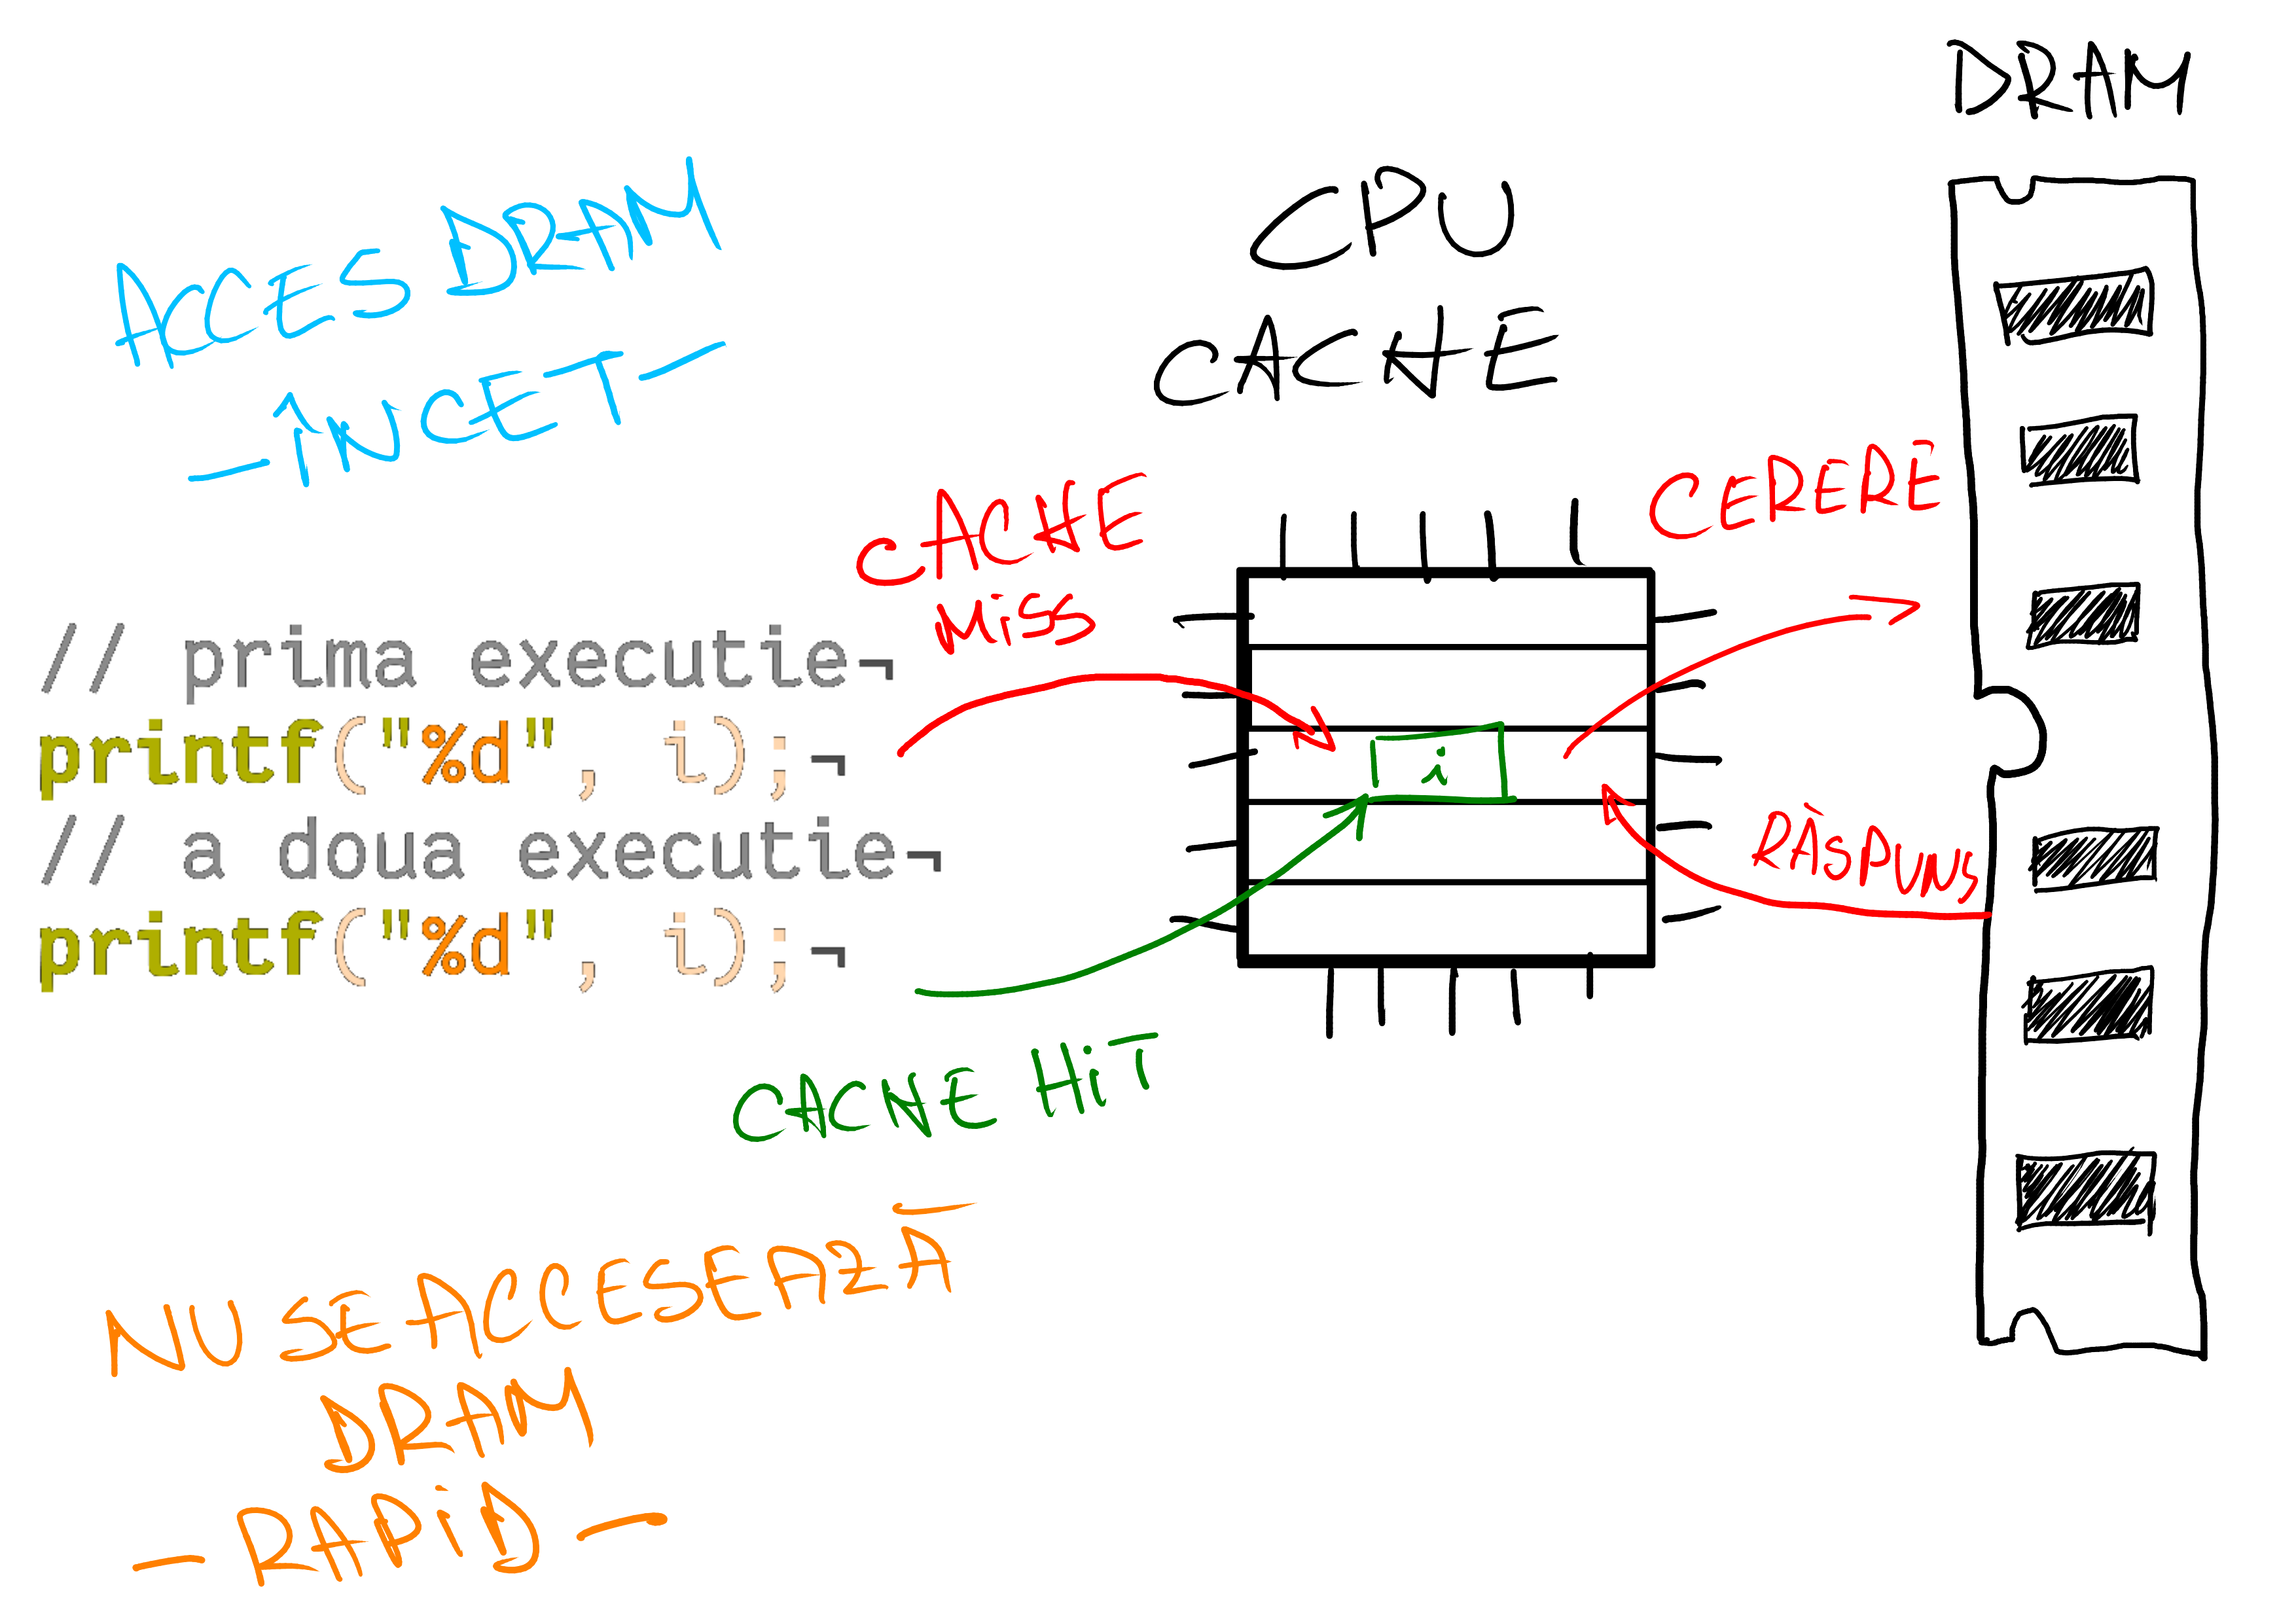
\includegraphics[width=0.9\textwidth]{images/cache_hit.png}
	\caption{Cache hit vs Cache miss}
  \label{fig:cache_hit}
\end{figure}

Timpul de accesare al valorii corespunzătoare variabilei \texttt{value} poate
fi calculat utilizând instrucțiunea \texttt{\_\_rdtscp} specifică procesoarelor
Intel. Aceasta permite citirea \emph{time-stamp counter-ului} din procesor
\cite{rdtscp}. Prin doua măsurători ce încadrează dereferentierea pointer-ului
către \texttt{value}, putem măsură numărul de ciclii de procesor necesari
operației. Repetând experimentul de $10000$ de ori și calculând media
timpului de acces pentru fiecare caz, se obțin următoarele rezultate:

\begin{itemize}
  \setlength\itemsep{0em}
  \item încărcarea din memorie durează aproximativ $250$ de ciclii și poartă
    numele de \emph{cache miss}
  \item încărcarea din cache durează aproximativ $23$ de ciclii și poartă
    numele de \emph{cache hit}
\end{itemize}

Aceste diferență măsurabile sunt exploatate în cadrul diferitelor
tehnici de atac asupra memoriei cache, printre care și \emph{FLUSH and RELOAD}
care vă fi discutat în continuare.

\subsubsection{Observație}

Numărul de ciclii de procesor necesari execuției unui set de instrucțiuni
diferă în funcție de sistem. Rezultatele ilustrate anterior sunt specifice unui
sistem ce rulează o versiune la zi a Kernelului Linux în data de
22.05.2022 (\texttt{Linux 5.17.9-arch1-1 x86\_64}), cu un procesor al
producătorului \emph{Intel}, modelul \texttt{i5-8250U} (mai multe specificații
pe site-ul producătorului \cite{i5_8250U}), cu 8GB de memorie RAM tip DDR3.

\subsubsection{FLUSH and RELOAD}\label{sec:flush_reload}

O practică comună de reducere a memoriei utilizate este partajarea între
procese a unor pagini comune cu drepturi exclusive de citire
(\emph{read-only}). \emph{FLUSH and RELOAD} este una dintre tehnicile
documentate de atac asupra memoriei cache. Scenariul descris în lucrarea de
cercetare în care a fost introdus atacul este acela al unei victime și al unui
spion care împart o zonă partajata de memorie. Spionul se folosește de
instrucțiunea \texttt{clflush} care invalidează liniile aferente unei zone de
memorie din toată ierarhia cache-ului din procesor \cite{clflush}, iar apoi
așteaptă o perioada scurta de timp. În final verifică daca la accesarea zonei
respective obține un \emph{cache hit} sau un \emph{cache miss}, astfel aflând
daca victima a accesat sau nu în fereastra respectivă de timp, zona de memorie
urmărită. Repetând experimentul, s-au putut extrage informații suficiente
pentru realizarea unor atacuri de succes asupra implementării de la vremea
respectiva a unor algoritmi criptografici (\emph{OpenSSL}, \emph{AES}),
monitorizarea activității unui utilizator, etc. \cite{flush_reload}.

\subsubsection{Alte tipuri de atacuri asupra memoriei cache}

\emph{FLUSH and FLUSH} se aseamănă cu \emph{FLUSH and RELOAD}, diferența 
constând în faptul că spionul în loc de a măsură timpul de acces a zonei
tintă, vă apela iarăși \texttt{clflush}. Execuția mai rapida vă corespunde
unui \emph{cache miss}, iar cea mai rapida unui \emph{cache hit} \cite{cache_attacks}.

\emph{EVICT and RELOAD} folosește un \emph{eviction set} pentru a elimina din
cache zona de memorie tintă. Apoi, pentru măsurarea timpului se procedează 
identic ca la \emph{FLUSH and RELOAD}. Tehnica se aseamănă în eficienta cu 
cele menționate anterior \cite{cache_attacks}.

\emph{PRIME + PROBE} constă într-o abordare diferita. Atacatorul umple toată
zona partajata din cache (\emph{PRIME}). Victima vă elimina valori încărcate
de atacator în cache în timp ce rulează (\emph{evict}). Atacatorul va măsura 
apoi timpul de acces pentru toată zona de cache (\emph{probe}). În cazul în care observă
un \emph{cache hit}, constată că victima a accesat zona respectivă \cite{cache_attacks}.

\subsection{Covert-channel}

Un \emph{cover channel} reprezintă un mod, sau protocol de comunicare ascuns.
Prin ascuns înțelegem că este foarte greu, sau chiar imposibil de detectat de
către un administrator, sau alți utilizatori de pe sistem, întrucât nu
presupune transmiterea de date într-un mod uzual. Utilizarea tehnicilor
descrise anterior pentru extragerea diverselor informații, fac ca memoria cache
să devină un astfel de canal de comunicare ascuns. Un astfel de mod de comunicare
poate fi utlizat pentru transmiterea de informații între procese care în mod normal
nu ar fi avut dreptul să comunice, conform politicilor de securitate prezente pe 
sistem \cite{covert_channel}. 

\subsection{Atacuri Speculative}

Atacurile Speculative se bazează pe exploatarea tehnicii de optimizare numită
\emph{Execuție Speculativă} care, datorită avantajelor aduse în performata,
este utilizată în prezent de majoritatea procesoarelor folosite în prezent.
Atacurite se folosesc de această optimizare pentru a produce intenționat efecte
secundare măsurabile, cu scopul de a accesa date în mod neautoriazat, prin
intermediul unor canale secundare (\emph{side channeles}) sau ascunse
(\emph{covert channels}). În continuarea acestei lucrări voi discuta
particularitățile și implicațiile câtorva atacuri din această clasă care au
avut un impact semnificativ asupra industriei în ultimii ani.

\subsection{ROP}\label{sec:rop}

\emph{ROP} \cite{shacham2007geometry} este o tehnica prin care un atacator care
reuseste sa deturneze fluxul normal de instructiuni, poate sa manipuleze
victima in realizarea unor actiuni complexe. In acest scop, atacatorul executa
in lant sevente reduse ca dimensiune de instructiuni masina numite
\emph{gadget-uri}. Gaget-urile sunt prezente si identificate de atacator in
codul sursa al victimei si se aseamana prin faptul ca realizeaza operatii
oarecare inaintea executarii unei instrutiuni (sau set de instructiuni) de tip
\emph{return}. Daca un atacator poate prelua controlul
\emph{stack-pointer-ului}, atunci poate redirectiona foluxul de instructiunui
catre un gadget special ales, care la randul lui va ridirectiona fluxul catre
alt gadget. S-a demonstrat ca un set restrans de gadget-uri poate fi echivalent
cu un limbaj Turing-Complete \cite{homescu2012microgadgets}. Pe idei preluate
din \emph{ROP} se bazeaza variante ale clasei de atacuri \emph{Spectre}, care
apeleaza in mod speculativ \emph{gadget-uri} din spatiul de meomorie al
victimei.

\begin{figure}[ht]
	\centering
	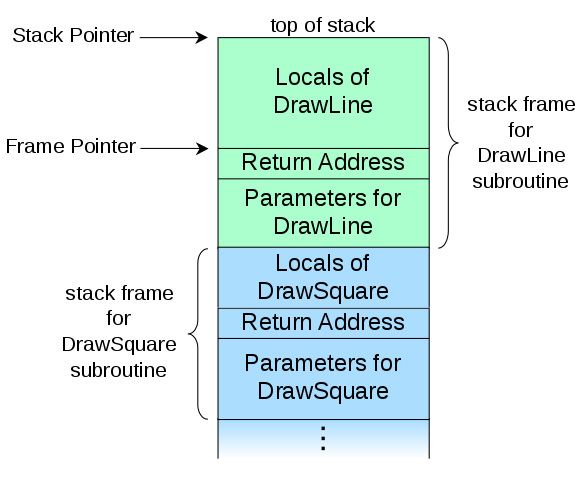
\includegraphics[width=0.9\textwidth]{images/rop_stack_layout.png}
  \caption{Stack Layout - ROP attack \cite{rop_figure}}
  \label{fig:rop_stack_layout}
\end{figure}
